% !TEX options=--shell-escape
% Beamer template by Julian Lueken

\documentclass[8pt, aspectratio=169]{beamer}
\usepackage[main=ngerman]{babel}
\usepackage[T1]{fontenc}
\usepackage{tikz}
\usepackage{helvet}
\usepackage{lipsum}
\usepackage{float}
\usepackage{svg}
\usepackage{subcaption}
\renewcommand{\familydefault}{\sfdefault}

\definecolor{mypres}{RGB}{97,107,104}

\makeatletter
\newcommand*\bigcdot{\mathpalette\bigcdot@{.5}}
\newcommand*\bigcdot@[2]{\mathbin{\vcenter{\hbox{\scalebox{#2}{$\m@th#1\bullet$}}}}}
\makeatother

% setting some colors for the theme
\setbeamercolor{palette primary}{fg=mypres,bg=white}
\setbeamercolor{palette secondary}{fg=mypres,bg=white}
\setbeamercolor{structure}{fg=mypres,bg=white}
\setbeamercolor{title in head/foot}{fg=black,bg=white}
\setbeamercolor{date in head/foot}{fg=gray,bg=white}

% definition of the headline template
\defbeamertemplate*{headline}{mytheme}{%
	\begin{tikzpicture}[remember picture, overlay]
		\node[text=mypres,anchor=west,font=\sffamily\tiny,text width=0.8\paperwidth] at ([xshift=7pt,yshift=0.5\textheight]current page.west) (header0) {DLR.de{ }$\bigcdot${ }Folie \insertframenumber};
		\node[text=mypres,anchor=west,font=\sffamily\tiny,text width=0.8\paperwidth] at ([xshift=55pt,yshift=0.5\textheight]current page.west) (header1) {$\bigcdot${ }\insertshorttitle{ }$\bigcdot${ }\insertauthor{ }$\bigcdot${ }\insertdate};
	\end{tikzpicture}
	\vskip15pt
}

% definition of the footline template arial
\defbeamertemplate*{footline}{mytheme}{%
	\begin{tikzpicture}[remember picture, overlay]
		\node[inner sep=0, anchor = south east] at (current page.south east) (banner) {
\includegraphics[page=1, width=\paperwidth]{footer.pdf}};
	\end{tikzpicture}
	\vskip0pt
}

% definition of the title page template
\defbeamertemplate*{title page}{mytheme}[1][] {
	\begin{tikzpicture}[remember picture, overlay]
		\node[text=mypres,anchor=west,font=\sffamily\tiny,text width=0.8\paperwidth] at ([xshift=6pt,yshift=0.5\textheight]current page.west) (header0) {DLR.de{ }$\bigcdot${ }Folie \insertframenumber};
		\node[text=mypres,anchor=west,font=\sffamily\tiny,text width=0.8\paperwidth] at ([xshift=54pt,yshift=0.5\textheight]current page.west) (header1) {$\bigcdot${ }\insertshorttitle{ }$\bigcdot${ }\insertauthor{ }$\bigcdot${ }\insertdate};
		\node[inner sep=0, anchor = south east] at (current page.south east) (banner) {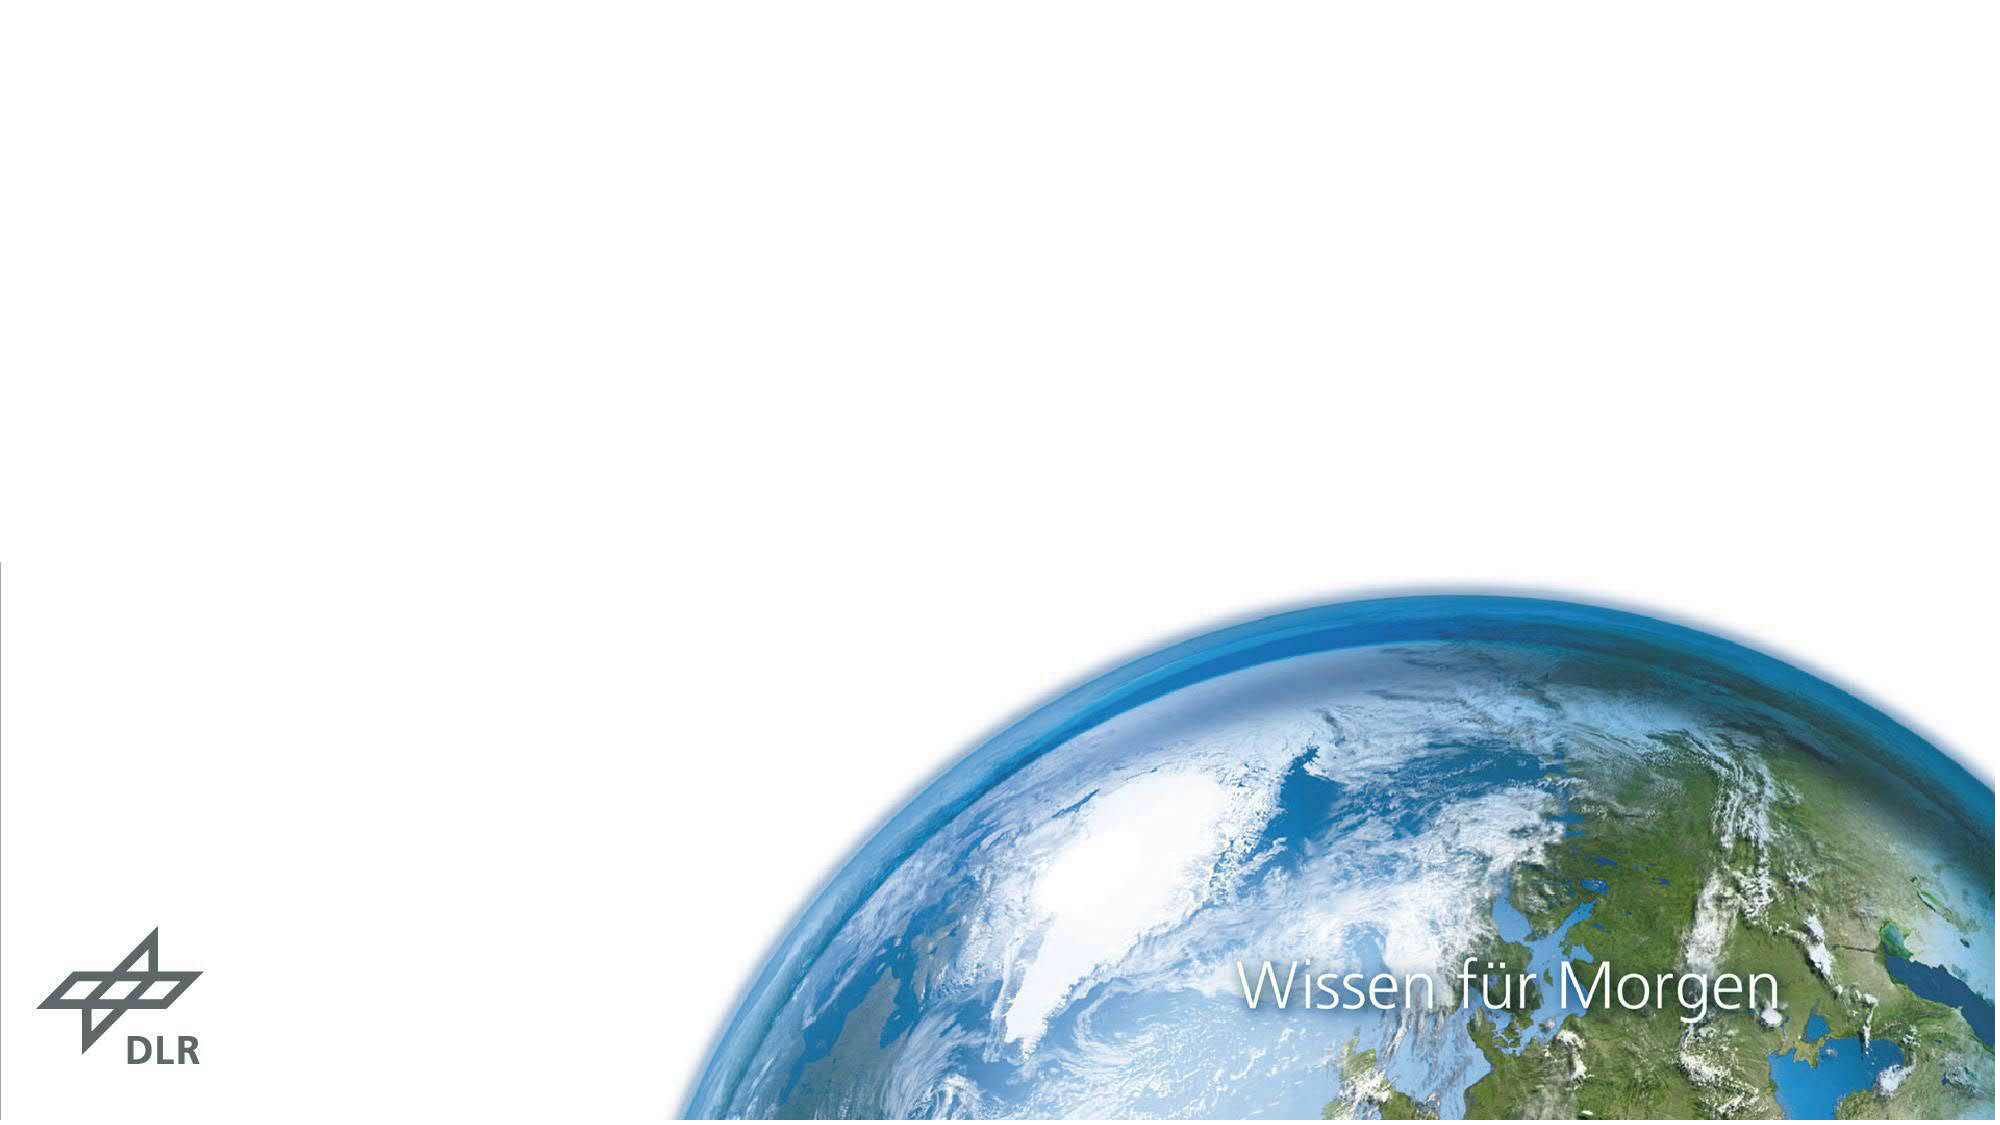
\includegraphics[page=1, width=\paperwidth]{header.pdf}};
		\node[text=mypres,anchor=south west,font=\sffamily\LARGE,text width=0.8\paperwidth] at ([xshift=7pt,yshift=1.50cm]current page.west) (title) {\raggedleft\insertshorttitle};
		\node[text=mypres,anchor=south west,font=\sffamily\large,text width=0.8\paperwidth] at ([xshift=7pt,yshift=1.00cm]current page.west) (subtitle) {\raggedleft\inserttitle};
		\node[text=mypres,anchor=south west,font=\sffamily,text width=.55\paperwidth] at ([xshift=7pt,yshift=-1cm]current page.west) (author) {\raggedright\insertauthor};
		\node[text=mypres,anchor=south west,font=\sffamily,text width=.55\paperwidth] at ([xshift=7pt,yshift=-1.5cm]current page.west) (date) {\raggedright\insertdate};
	\end{tikzpicture}
	\vskip0pt
}

% remove navigation symbols
\setbeamertemplate{navigation symbols}{}

\title[CoolingGen]{Eine Software zur Erstellung von Kühlungsgeometrien}
\author{Julian Lüken}
\date{\today}

\begin{document}

\begin{frame}[plain]
	\maketitle
\end{frame}

\begin{frame}
	\frametitle{Einleitung/Motivation}
	\vspace{-1cm}\hspace{-0.5cm}
	\begin{minipage}[t]{\textwidth}
		Was ist CoolingGen?
		\begin{itemize}
			\item Programm, welches mithilfe von CAD eine Schaufel aus BladeGen mit Kühlungsgeometrien ausstattet
			\item Basiert auf BasicTools (Bibiliothek vom DLR für B-Spline Kurven/Flächen)
			\item Entwicklung startete 2013 (Autoren: C. Voß, T. Schumacher)
			\item Meine Arbeit daran startete im Juli 2021
		\end{itemize}
		\vspace{0.5cm}
		Warum CoolingGen?
		\begin{itemize}
			\item Erzeugung von Kühlungsgeometrien innerhalb einer Schaufel mit herkömmlichen CAD-Tools ist mühsam und dauert lange
			\item Laufzeit von CoolingGen: ca. 20 Sekunden auf 8 $\cdot$ 3GHz
			\item Grundlage für die Optimierung von Kühlungsgeometrien durch Phasenraumsuche gekoppelt mit CFD-Simulationen
		\end{itemize}

	\end{minipage}
	\vfill
\end{frame}

\begin{frame}
	\frametitle{Einleitung/Motivation}
	\vspace{-1cm}\hspace{-0.5cm}
	\begin{minipage}[t]{\textwidth}
		Input:
		\begin{itemize}
			\item Schaufelgeometrie aus BladeGen
			\item Parameter für die Kühlungsgeometrien (als XML)
		\end{itemize}
		Output:
		\begin{itemize}
			\item Kühlungsgeometrien (als STEP, für CENTAUR und für Tecplot)
		\end{itemize}

		Welche Geometrien kann CoolingGen erzeugen?
		Derzeit unterstützt (und hier vorgestellt):
		\begin{itemize}
			\item Kühlkanäle (mit Umkehrungen)
			\item Prallbleche (mit Bohrungen)
			\item Filmkühlung
		\end{itemize}

		To-do:
		\begin{itemize}
			\item Ausblasungsschlitze
			\item Pin-fins
		\end{itemize}
	\end{minipage}
	\vfill
\end{frame}

\begin{frame}
	\frametitle{Ergebnisse}
	\vspace{-1cm}\hspace{-0.5cm}
	\begin{figure}
		\centering
		\begin{subfigure}[t]{.49\textwidth}
			\centering
			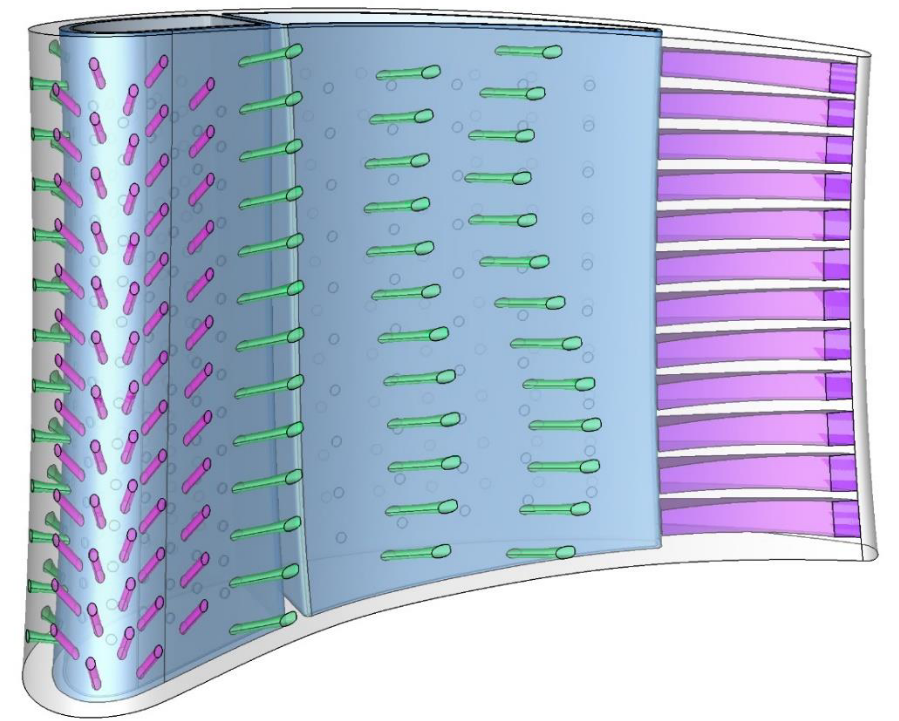
\includegraphics[height=.6\textheight]{../tec/complete/17.png}
		\end{subfigure}
		\begin{subfigure}[t]{.49\textwidth}
			\centering
			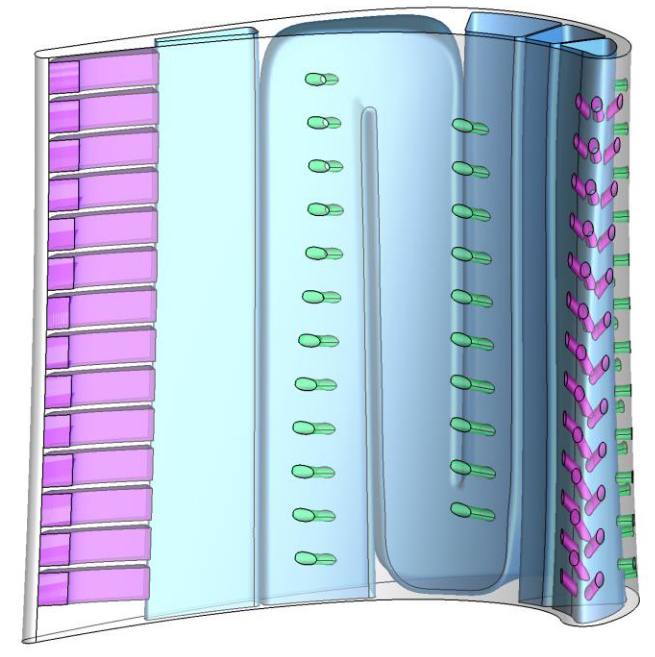
\includegraphics[height=.6\textheight]{../tec/complete/18.png}
		\end{subfigure}
	\end{figure}
	\vfill
\end{frame}

\begin{frame}
	\frametitle{Methoden / Kanäle und Prallbleche}
	\vspace{-1cm}\hspace{-0.5cm}
	\begin{minipage}[t]{\textwidth}
		Um die Kanäle zu erzeugen, werden $m$ Kanalwände (in Relation zur Skelettlinie) als Input spezifiziert.
		Es wird folgende Strategie verwendet:
		\begin{enumerate}
			\item Schaufeloberfläche in radialer Höhe $n$ mal samplen $\rightarrow$ $n$ Profilkurven
			\item Koordinatentransformation $(x, y, z) \rightarrow (x, r) \rightarrow (m', \theta)$
			\item \emph{Schrumpfen} der Profilkurven
			\item \emph{Unterteilung} der Profilkurven an den Kanalwänden $\rightarrow$ $n(m+1)$ Kammerschnitte 
			\item \emph{Schrumpfen} der Kammerschnitte
			\item Einpassung von \emph{Fillets} an \emph{Knicken/Ecken}
			\item Rücktransformation nach $(x, y, z)$, und \emph{Lifting}, um $m+1$ Oberflächen zu erhalten
		\end{enumerate}
	\end{minipage}
	\vfill
\end{frame}

\begin{frame}
	\frametitle{Methoden / Kanäle und Prallbleche / Schrumpfen der Profilkurven}
	\vspace{-1cm}\hspace{-0.5cm}
	\begin{figure}
		\centering
		\begin{subfigure}[t]{.49\textwidth}
			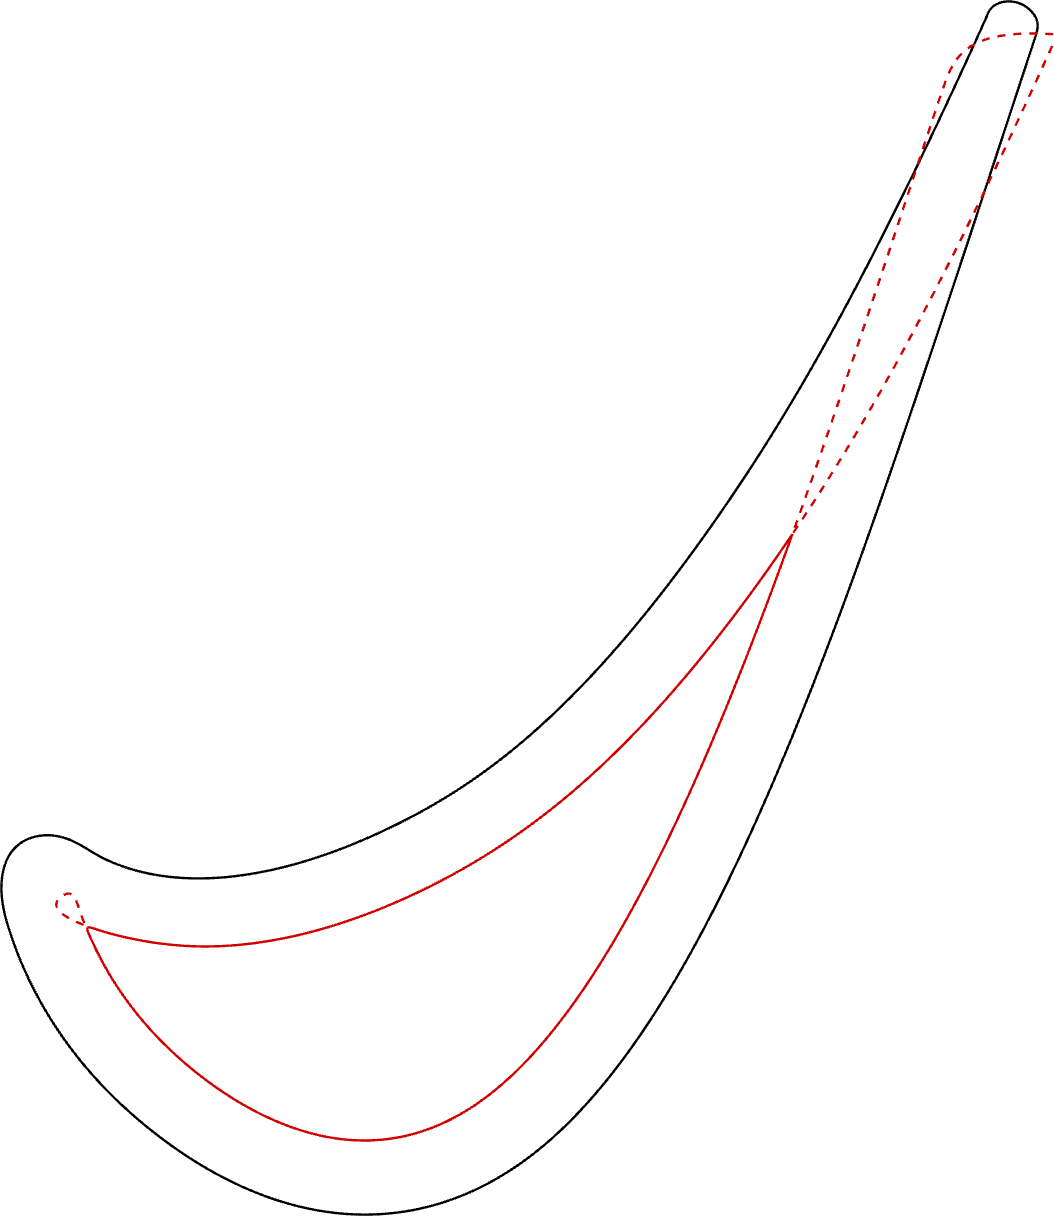
\includegraphics[height=.8\textheight]{../tec/shrinking/offset.png}
		\end{subfigure}
		\begin{subfigure}[t]{.49\textwidth}
			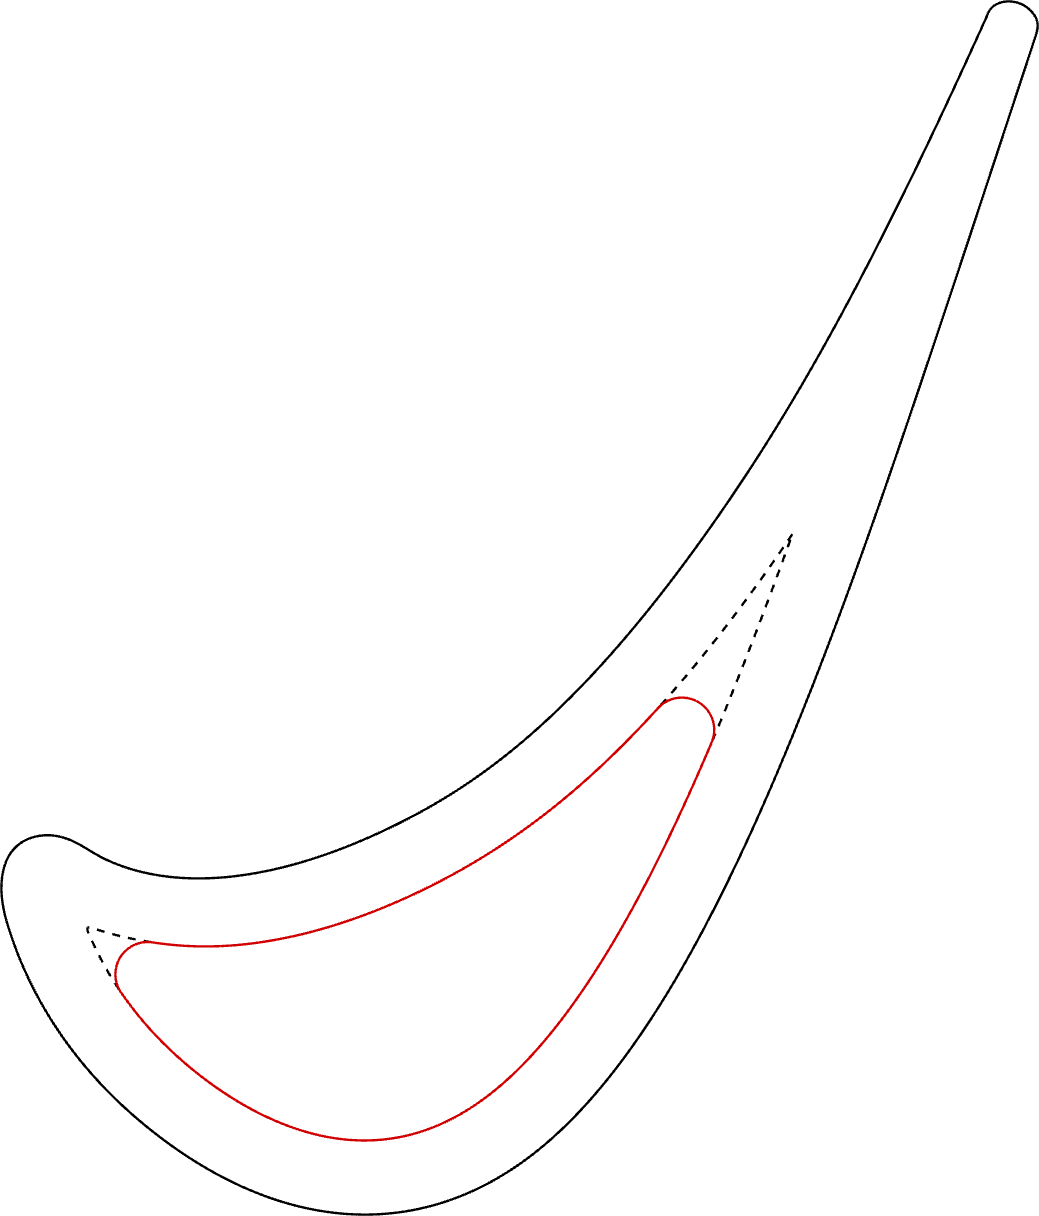
\includegraphics[height=.8\textheight]{../tec/shrinking/trimming.png}
		\end{subfigure}
	\end{figure}
\end{frame}

\begin{frame}
	\frametitle{Methoden / Kanäle und Prallbleche / Offset-Kurven}
	\vspace{-1cm}\hspace{-0.5cm}
	\begin{minipage}[t]{\textwidth}
		Eine Offset-Kurve von $\gamma$ mit Abstand $d$ ist gegeben durch
			$$ O^\gamma_d(t) := \gamma(t) + dN^\gamma(t)$$
		wobei $N^\gamma(t)$ der Normalenvektor von $\gamma(t)$ ist.
	\end{minipage}
	\begin{figure}[H]
		\centering
		\begin{subfigure}{0.49\textwidth}
			\includesvg[width=0.98\textwidth]{../python/offsetCurveSelfIntersection0}
		\end{subfigure}
		\begin{subfigure}{0.49\textwidth}
			\includesvg[width=0.98\textwidth]{../python/offsetCurveSelfIntersection1}
		\end{subfigure}
	\end{figure}
	\hspace{-0.5cm}
	\begin{minipage}[t]{\textwidth}
		Wir hätten die Kurve $O^\gamma_d$ gerne injektiv. Das gilt jedoch nur stückweise $\rightarrow$ Trimming an Selbstschnittpunkten.\\
		Das Trimming hinterlässt nicht diff'bare Stellen (Knicke) $\rightarrow$ Fillets!
	\end{minipage}
\end{frame}

\begin{frame}
	\frametitle{Methoden / Kanäle und Prallbleche / (Selbst-)Schnittpunkte von Kurven}
	\vspace{-0.5cm}\hspace{-0.5cm}
	\begin{minipage}[t]{\textwidth}
		Lineare Approximation der Kurven schneiden ist relativ einfach $\rightarrow$ Teile und herrsche.
		\begin{figure}[H]
			\centering
			\includesvg[width=0.98\textwidth]{../python/piecewiseLinearIntersection}
		\end{figure}
	\end{minipage}
\end{frame}

\begin{frame}
	\frametitle{Methoden / Kanäle und Prallbleche / Fillets}
	\vspace{-0.5cm}\hspace{-0.5cm}
	\begin{minipage}[t]{\textwidth}
		Gegeben: Radius $r$, Kurven $\gamma_1, \gamma_2$. Man kann zeigen: Falls ein Filletkreis existiert, dann beschreibt
			$$ O^{\gamma_1}_r(t) = O^{\gamma_2}_r(s)$$
		den Mittelpunkt (bzw. die Mittelpunkte). Beweis gibt es in meiner Masterarbeit.
		\begin{figure}[H]
			\centering
			\includesvg[width=0.9\textwidth]{../python/filletConstruction1}
			\label{fig:filletconstruction}
		\end{figure}
		\begin{figure}[H]
			\centering
			\includesvg[width=0.9\textwidth]{../python/filletConstruction2}
		\end{figure}
	\end{minipage}
\end{frame}

\begin{frame}
	\frametitle{Methoden / Kanäle und Prallbleche / Unterteilung}
	\vspace{-1cm}\hspace{-0.5cm}
	\begin{figure}
		\centering
		\begin{subfigure}[t]{.5\textwidth}
			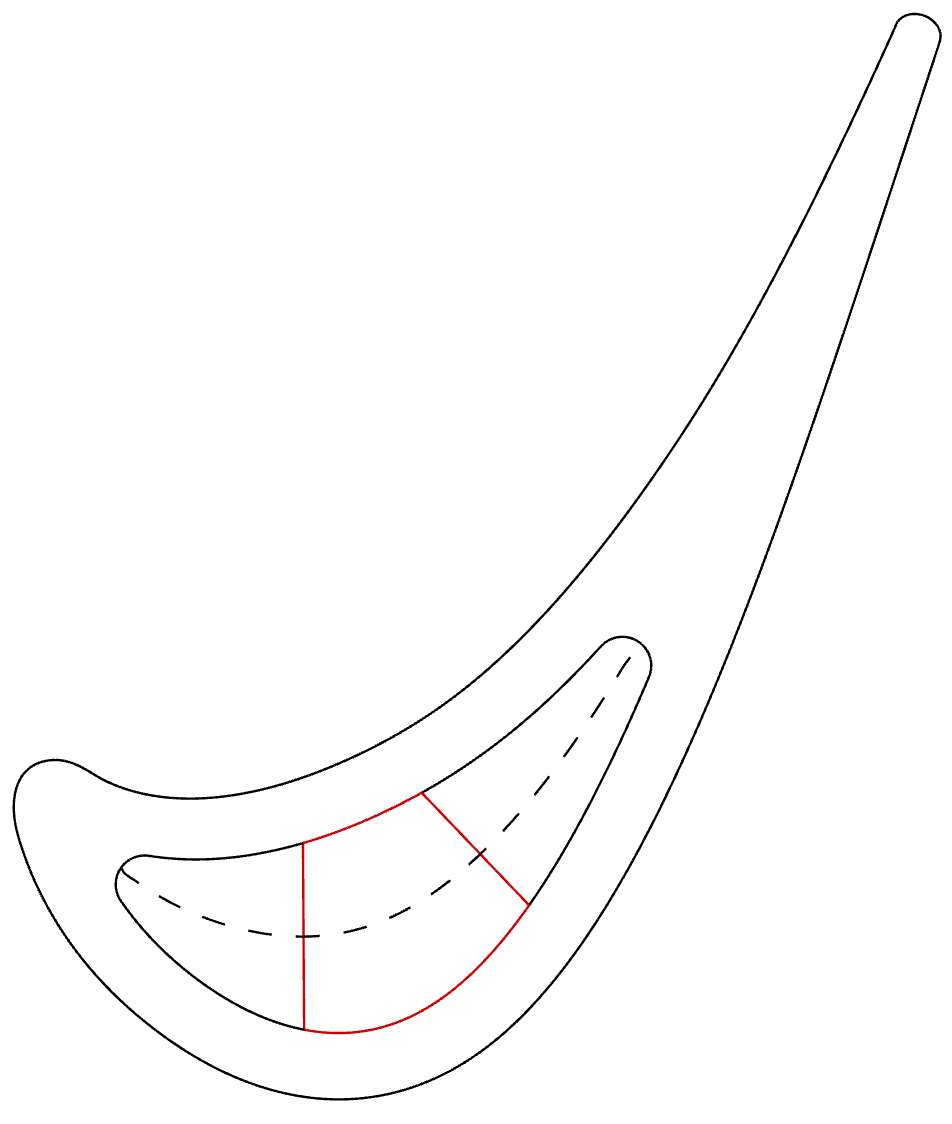
\includegraphics[height=.8\textheight]{../tec/chambers/walls.png}
		\end{subfigure}
		\begin{subfigure}[t]{.48\textwidth}
			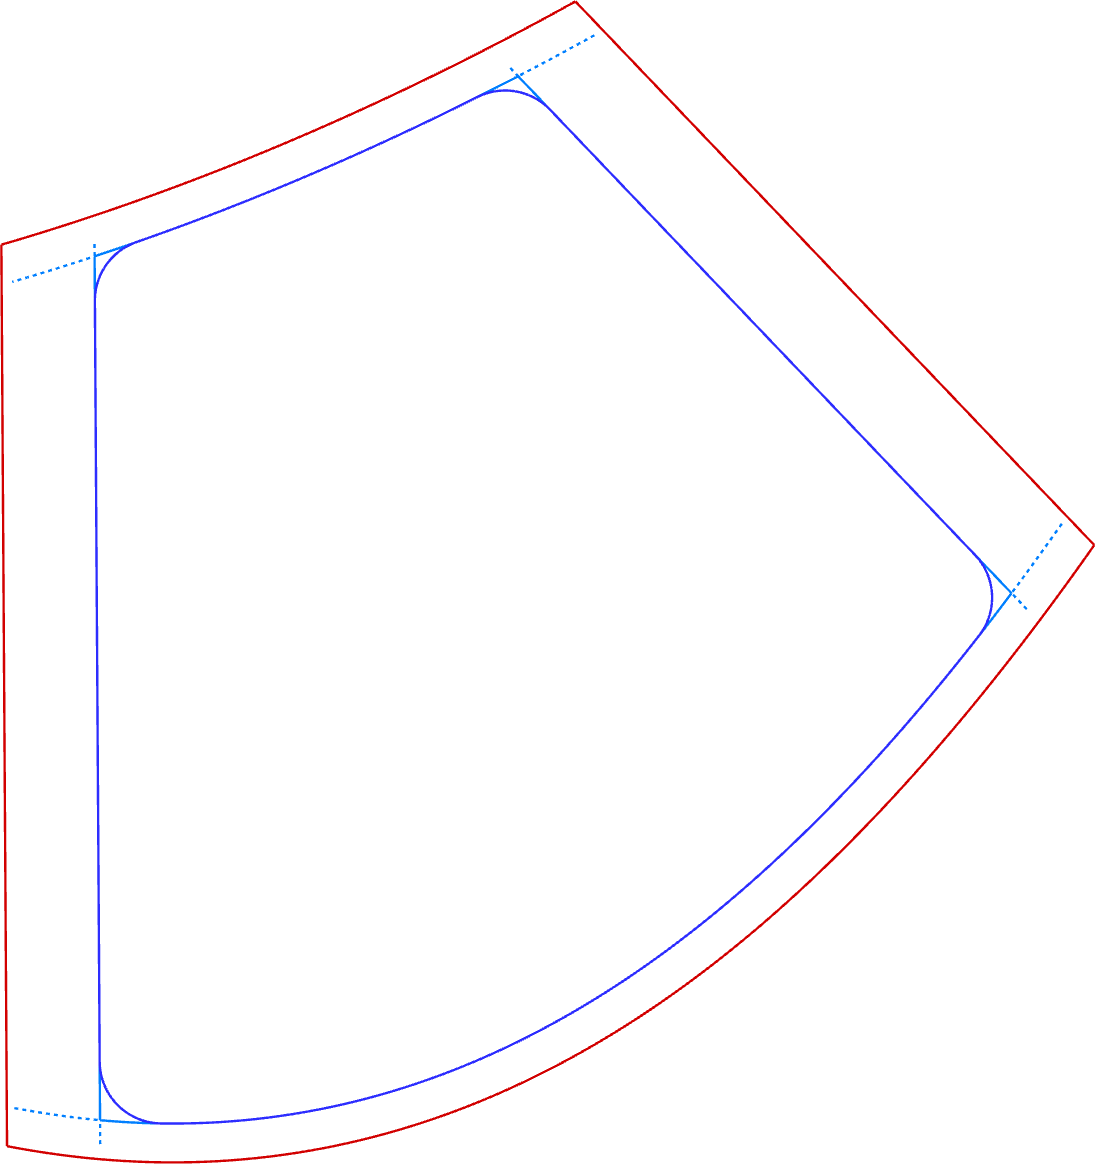
\includegraphics[height=.8\textheight]{../tec/chambers/single_constr.png}
		\end{subfigure}
	\end{figure}
\end{frame}

\begin{frame}
	\frametitle{Methoden / Kanäle und Prallbleche / Ray-Marching}
	\hspace{-0.5cm}
	Gegeben Kurve $\gamma$ und Halberade mit Startpunkt $A$ und normiertem Richtungsvektor $B$.\\
	Schnittpunktsuche durch folgenden Algorithmus:
	\begin{minipage}{\textwidth}
		\begin{figure}[H]
			\centering
			\includesvg[width=0.8\textwidth]{../python/rayMarching}
		\end{figure}
	\end{minipage}
\end{frame}

\begin{frame}
	\frametitle{Methoden / Kanäle und Prallbleche / Lifting}
	\vspace{-1cm}\hspace{-0.5cm}
	\begin{minipage}{\textwidth}
		\begin{figure}[H]
			\centering
			\begin{subfigure}{0.49\textwidth}
				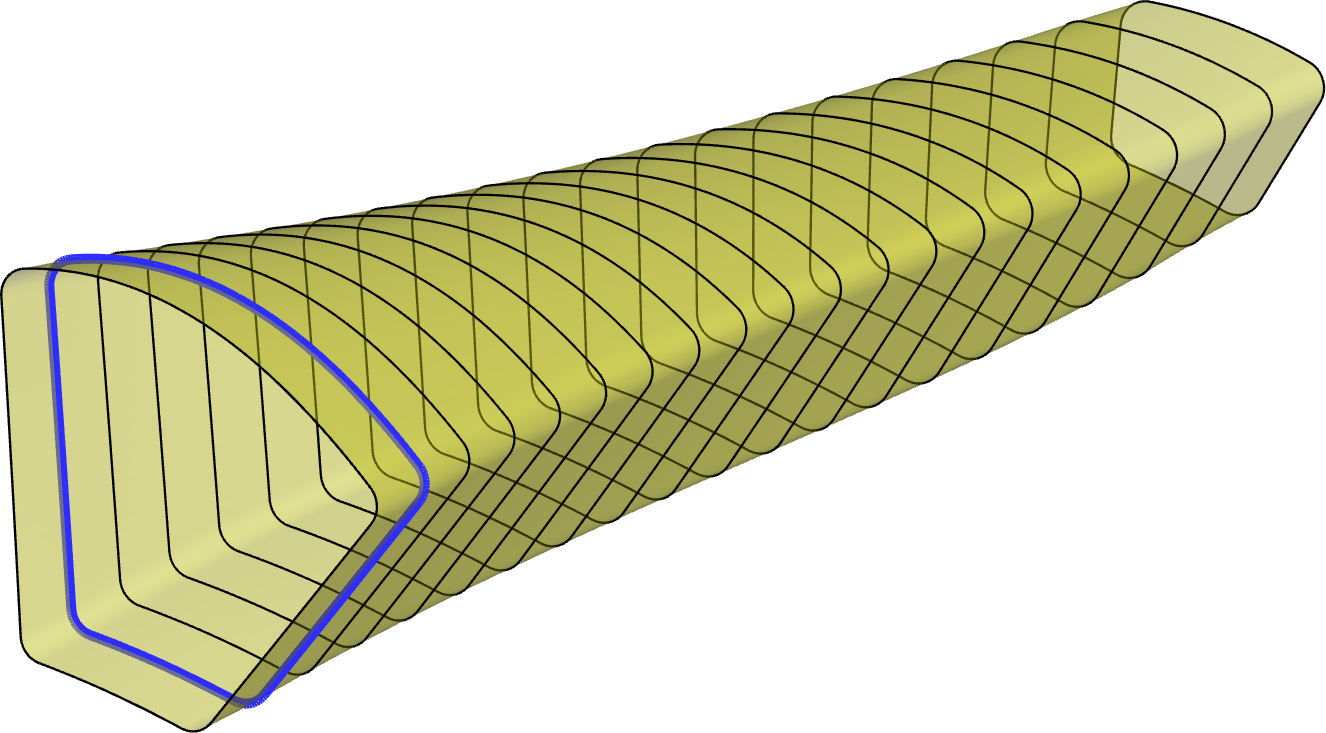
\includegraphics[width=\textwidth]{../tec/lifting/lifted.png}
				\vspace{1cm}
			\end{subfigure}
			\hspace{0.5cm}
			\begin{subfigure}{0.42\textwidth}
				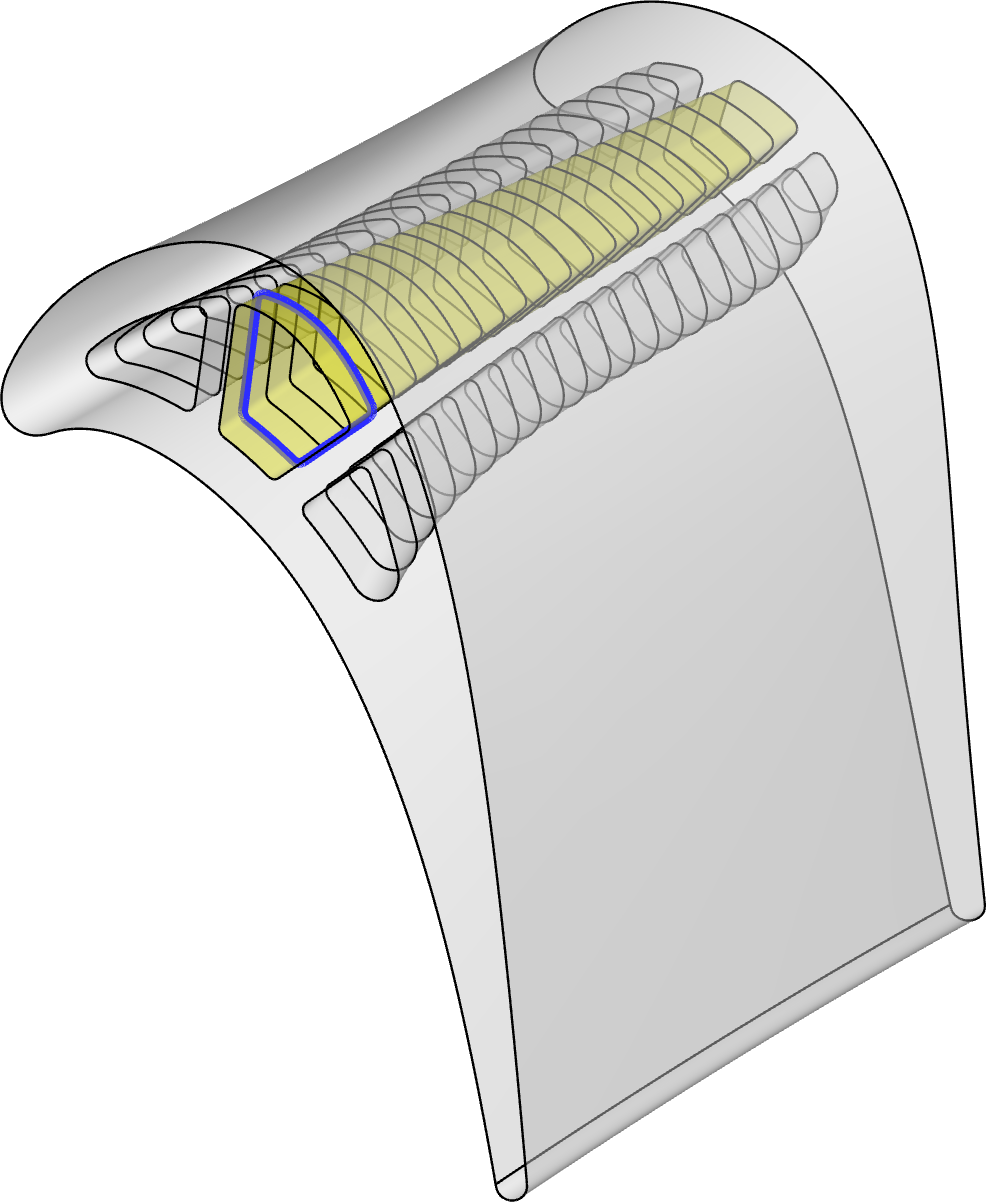
\includegraphics[width=\textwidth]{../tec/lifting/complete.png}
			\end{subfigure}
		\end{figure}
	\end{minipage} 
\end{frame}

\begin{frame}
	\frametitle{Methoden / Umkehrungen}
	\vspace{-1cm}\hspace{-0.5cm}
	\begin{minipage}[t]{\textwidth}
		Strategie:
		\begin{enumerate}
			\item Berechnung einer Kombination aus den zwei Kanälen, die sich zur Umkehrung verbinden
			\item Schneiden der kombinierten Kanäle mit $n$ Ebenen $\rightarrow$ $n$ planare Profilkurven
			\item Verformen der $n$ Kurven
			\item Lifting
		\end{enumerate}
	\end{minipage}
\end{frame}

\begin{frame}
	\frametitle{Methoden / Umkehrungen / Kombination}
	\vspace{-1cm}\hspace{-0.5cm}
	\begin{figure}
		\centering
		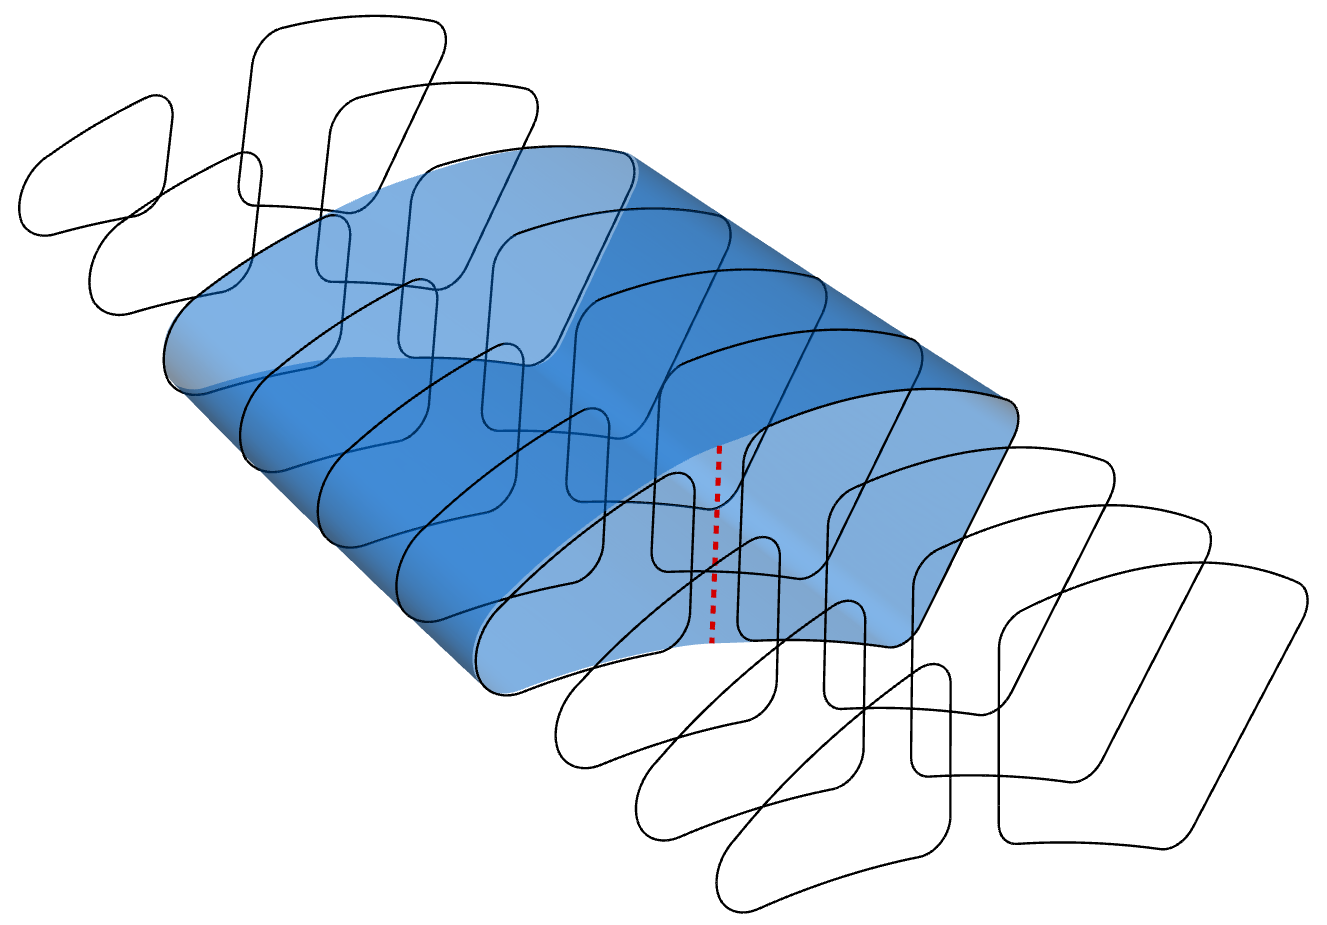
\includegraphics[height=.8\textheight]{../tec/turn/12.png}
	\end{figure}
\end{frame}

\begin{frame}
	\frametitle{Methoden / Umkehrungen / Verschneiden}
	\vspace{-1cm}\hspace{-0.5cm}
	\begin{figure}
		\centering
		\begin{subfigure}{.49\textwidth}
			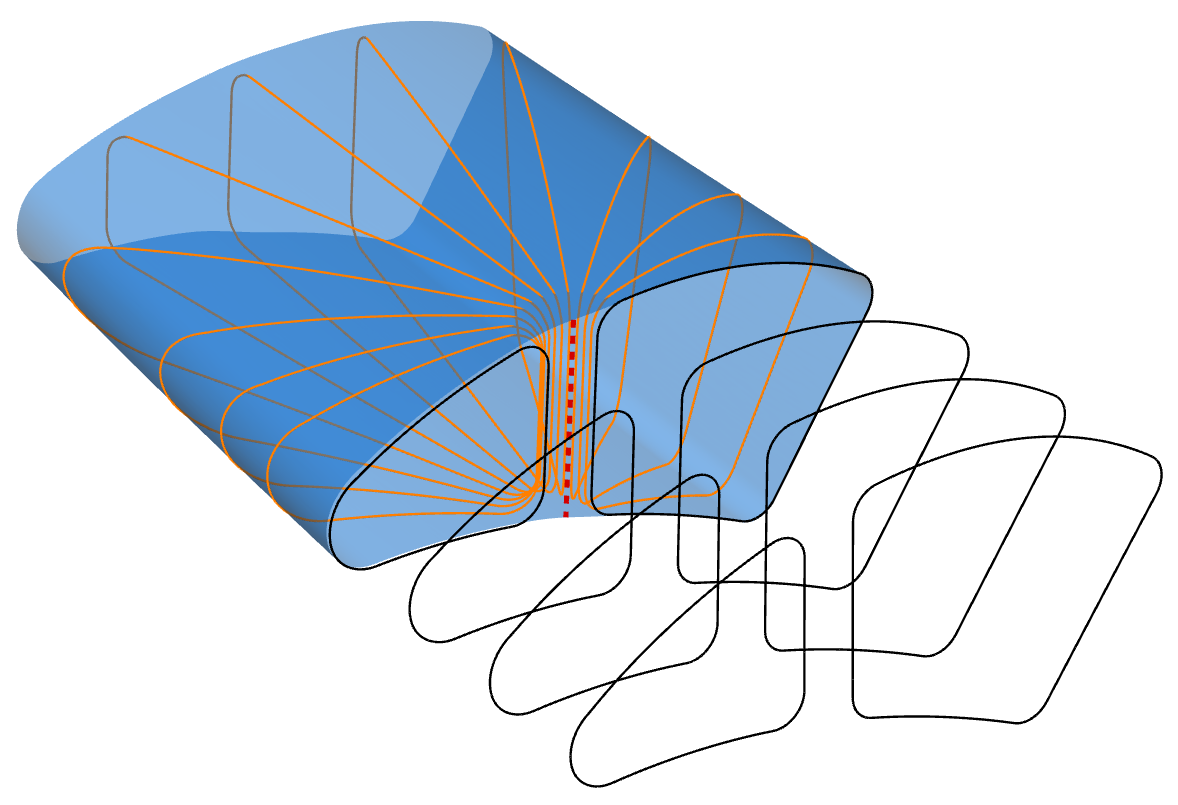
\includegraphics[width=\textwidth]{../tec/turn/11.png}
		\end{subfigure}
		\begin{subfigure}{.49\textwidth}
			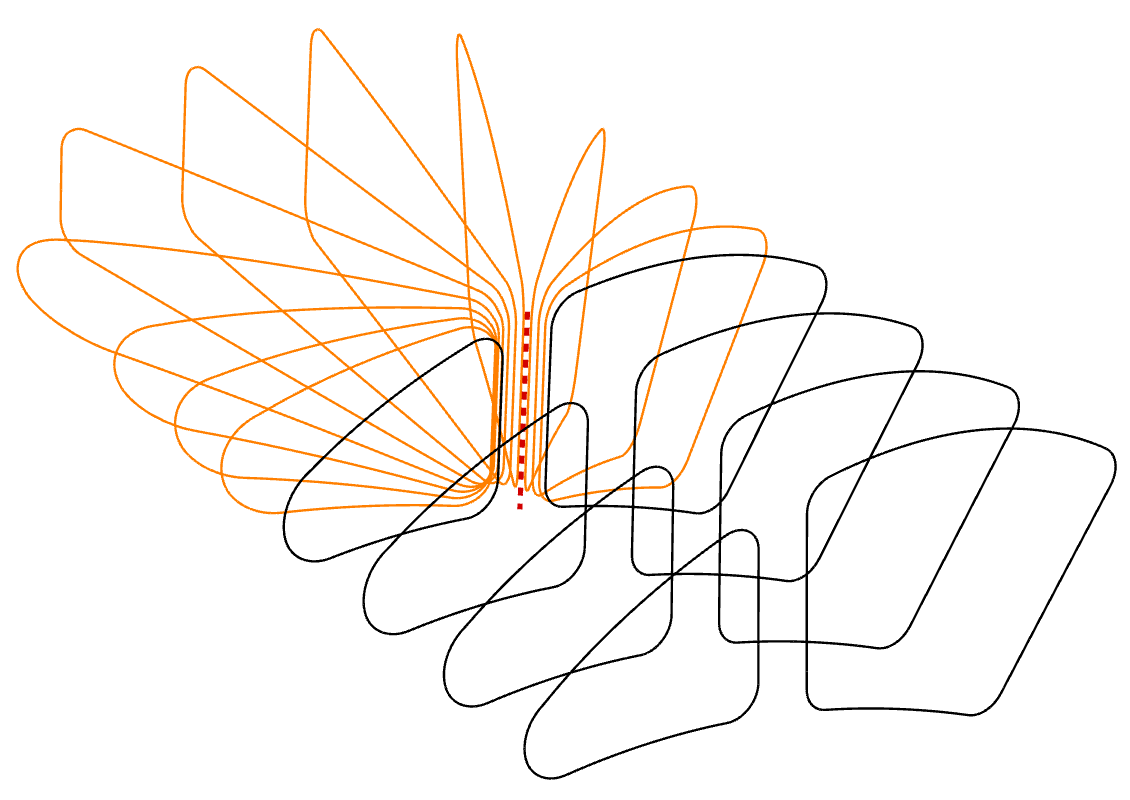
\includegraphics[width=\textwidth]{../tec/turn/10.png}
		\end{subfigure}
	\end{figure}
\end{frame}

\begin{frame}
	\frametitle{Methoden / Kanäle}
	\vspace{-1cm}\hspace{2.5cm}
	\begin{figure}
		\centering
		\begin{subfigure}{.49\textwidth}
			\phantom{aaaaaaa}
			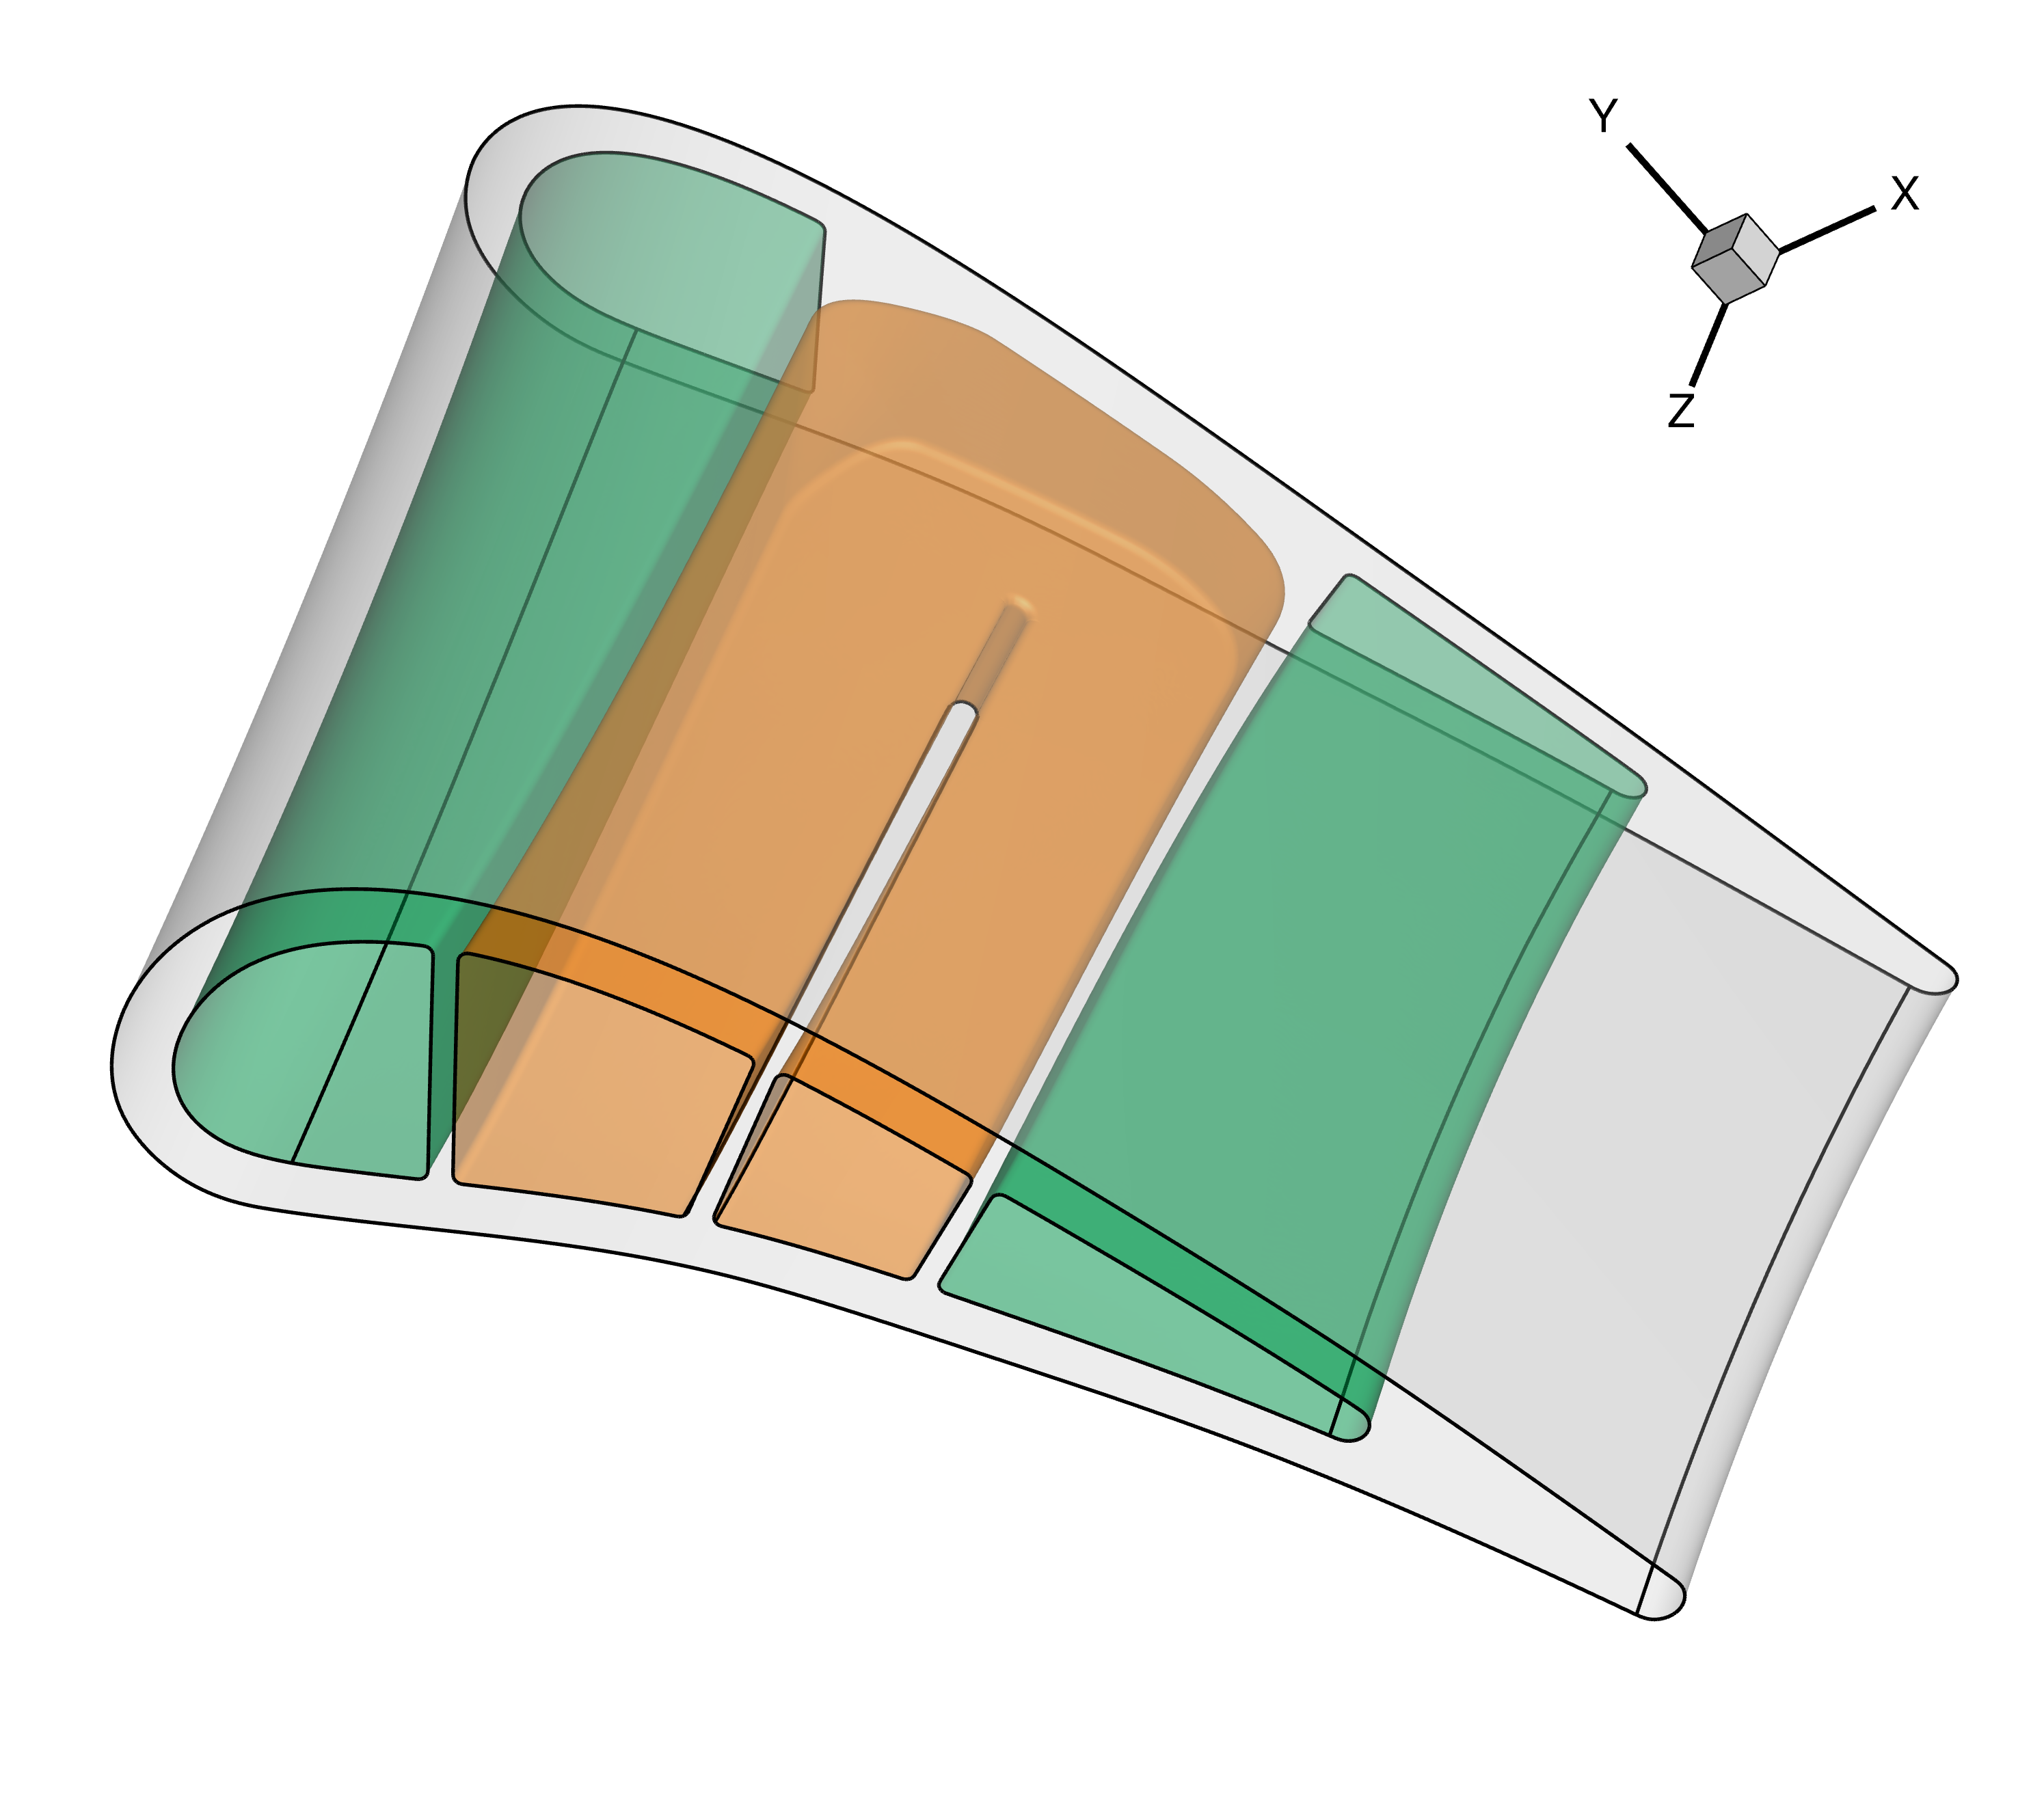
\includegraphics[height=.8\textheight]{../tec/channel/14.png}
		\end{subfigure}
		\begin{subfigure}{.49\textwidth}
			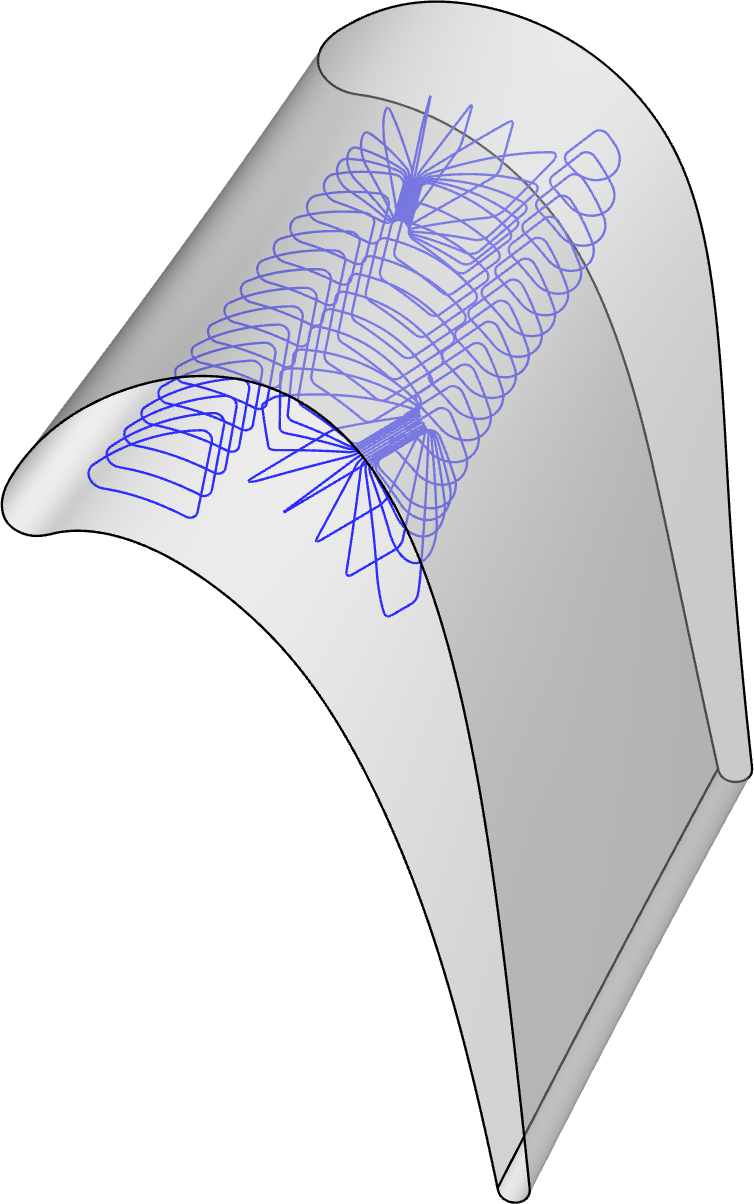
\includegraphics[height=.8\textheight]{../tec/channel/13.png}
		\end{subfigure}
	\end{figure}
\end{frame}

\begin{frame}
	\frametitle{Methoden / Bohrungen}
	\vspace{-1cm}\hspace{2.5cm}
	\begin{figure}
		\centering
		\begin{subfigure}{.3\textwidth}
			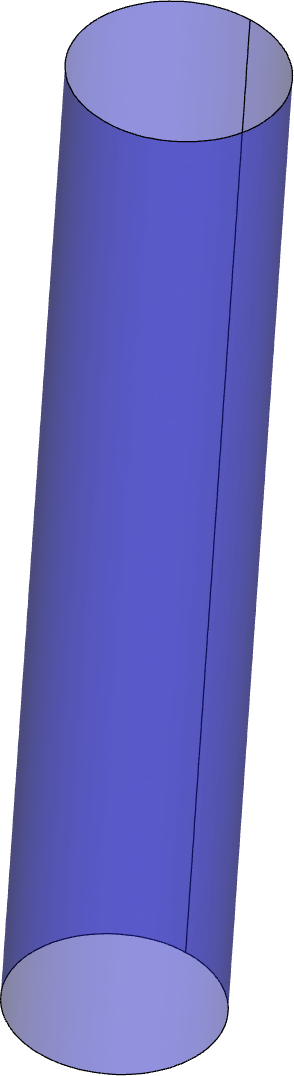
\includegraphics[height=.7\textheight]{../tec/holes/16.png}
		\end{subfigure}
		\begin{subfigure}{.3\textwidth}
			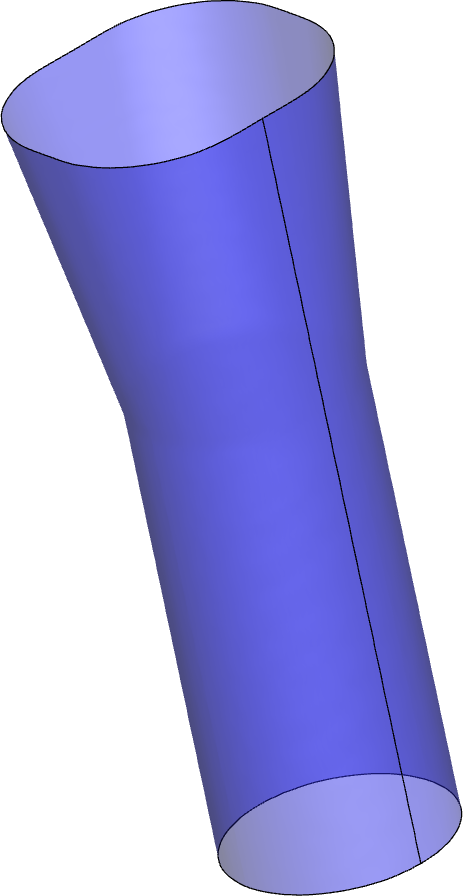
\includegraphics[height=.7\textheight]{../tec/holes/15.png}
		\end{subfigure}
		\begin{subfigure}{.3\textwidth}
			\includesvg[height=.7\textheight]{../python/fanshapedCurveDefinition}
		\end{subfigure}
	\end{figure}
\end{frame}

\begin{frame}
	\frametitle{Methoden / Fazit}
	\vspace{-1cm}\hspace{-0.5cm}
	\begin{minipage}[t]{\textwidth}
		\begin{center}
		Größte Herausforderung? Robuste und performante Verschnittalgorithmen!
		\end{center}
		\vspace{0.5cm}
		\begin{center}
		\emph{\glqq The single greatest cause of poor reliability of CAD systems is lack of topologically consistent surface intersection algorithms.\grqq}
		\end{center}
		\vspace{0.5cm}
		\flushright -- R. Farouki in \emph{\glqq Closing the Gap Between CAD Model and Downstream Applications\grqq}
	\end{minipage}
\end{frame}

\begin{frame}
	\frametitle{Ergebnisse}
	\vspace{-1cm}\hspace{-0.5cm}
	\begin{figure}
		\centering
		\begin{subfigure}[t]{.49\textwidth}
			\centering
			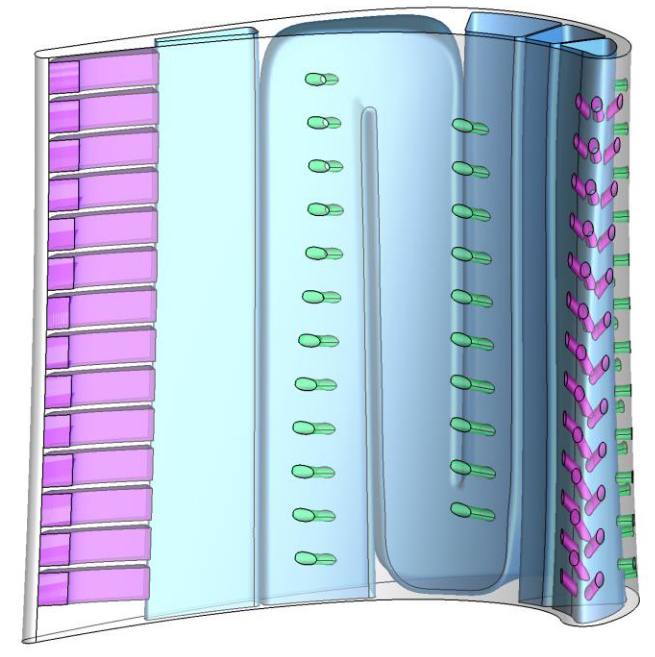
\includegraphics[height=.6\textheight]{../tec/complete/18.png}
		\end{subfigure}
		\begin{subfigure}[t]{.49\textwidth}
			\centering
			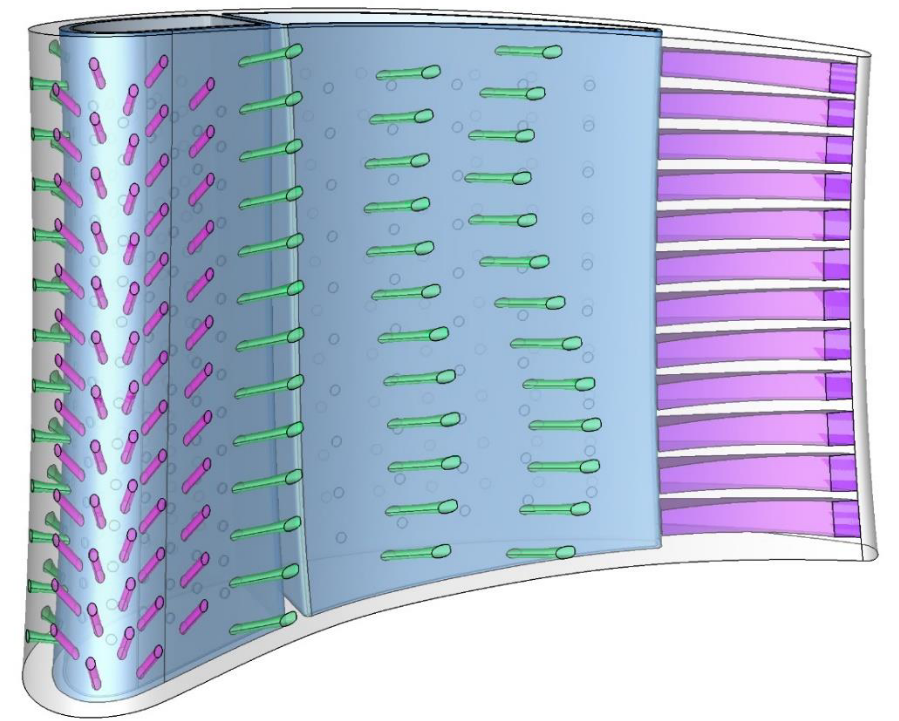
\includegraphics[height=.6\textheight]{../tec/complete/17.png}
		\end{subfigure}
	\end{figure}
	\vfill
\end{frame}

\begin{frame}
	\frametitle{}
	\begin{minipage}[t]{\textwidth}
		\centering
		\Large Fragen/Anmerkungen?
	\end{minipage}
\end{frame}

\end{document}